
\documentclass[12pt,journal,compsoc]{IEEEtran}
\ifCLASSOPTIONcompsoc
  % IEEE Computer Society needs nocompress option
  % requires cite.sty v4.0 or later (November 2003)
  % \usepackage[nocompress]{cite}
\else
  % normal IEEE
  % \usepackage{cite}
\fi

% *** GRAPHICS RELATED PACKAGES ***
%
\usepackage{float}

\ifCLASSINFOpdf
  \usepackage[pdftex]{graphicx}

\else

\fi

\newcommand\MYhyperrefoptions{bookmarks=true,bookmarksnumbered=true,
pdfpagemode={UseOutlines},plainpages=false,pdfpagelabels=true,
colorlinks=true,linkcolor={black},citecolor={black},urlcolor={black},
pdftitle={Memory Constraints and Solutions for Heterogeneous SoC},%<!CHANGE!
pdfsubject={Typesetting},%<!CHANGE!
pdfauthor={Michael D. Shell},%<!CHANGE!
pdfkeywords={Computer Society, IEEEtran, journal, LaTeX, paper,
             template}}%<^!CHANGE!

% correct bad hyphenation here
\hyphenation{op-tical net-works semi-conduc-tor}

\begin{document}
%
% paper title
% can use linebreaks \\ within to get better formatting as desired
% Do not put math or special symbols in the title.
\title{Memory Constraints and Solutions \\ for Heterogeneous SoC}

\author{The authors}

% The paper headers
\markboth{}%
{Shell \MakeLowercase{\textit{et al.}}: Bare Advanced Demo of IEEEtran.cls for Journals}
% The only time the second header will appear is for the odd numbered pages

\maketitle

\IEEEdisplaynontitleabstractindextext

\IEEEpeerreviewmaketitle

\section{Introduction}

\indent Recent developments start to show a modest but solid deviation to the well-known Gordon Moore's 40-year old law that talks about performance improvement in CPU processing power. Even though the mentioned law got several interpretations, only one seems to be able to keep up with the projected trend: the increase in number of transistor per die area (expected to double every 18-24 months). However, as we approach the limits of current Silicon manufacturing technologies, even that trend is threatened to flatten, not only because of the pure physical constraints (we are reaching manufacturing precisions of atoms), but also because of the more significant quantum phenomena that starts to be exhibited when talking about devices like SET (single-electron transistors).

One of the most important aspects left aside in the childhood of computing ages was the memory-barrier, probably the biggest constraint a computing system faces nowadays. There is a well known chart that addresses this issue, which shows that the memory - CPU gap also grows at an exponential rate. In other terms, this issue has a massive impact in CPU performance and further threatens to clutter the horizon of exponential innovation for the field of artificial intelligence and computing systems.

The complexity of the issue grows further with recent developments with heterogeneous SoC, because of integrating a bandwidth-hungry multi-core GPU on the same die. Although a higher level of integration can provide improvements in many areas, such as portability, power-efficiency and cost-efficiency, the bandwidth and latency challenges still remain and can truly bottleneck one of the two main components, regarding the provided scenario.


\section{Problems}
The main part of a conventional computing system architecture is comprised of a computing unit, it's physical memory, virtual memory and the data transfer buses between all of them. In order to keep up with the evolving state of processing power, memory hierarchy started to become more complex. Nowadays, SoCs include up to three levels of Cache memory, built as SRAM memory. The cache is tightly coupled with the compute units and is usually structured in two levels (L1 and L2). After 2003, Intel also integrated the LLC (last-level cache - also referred as L3) on the chip die, forcing motherboard vendors to remove it from their products. This solution reduced the latency and provided space for higher bandwidth, while decreasing miss rate slowdown.

As of 2009, for means of tighter integration and power consumption, consumer CPUs have started to engulf some GPU processing cores. The solution brought many innovations in the field, but also gave birth to several challenges to computer engineers and software architects. 

The biggest problems of such a high-level of integration are the memory management, bandwidth and latency. The issue grows further in complexity because the memory requirements do not scale in a linear manner, but more agressively due to the combined needs the two processors exhibit (the GPU and CPU); while the conventional main-purpose processor needs low-latency memory and moderate bandwidth, the GPU is not affected by a high latency, while the bandwidth requirements can be an order of magnitude bigger. 
\subsection{DRAM limitations in mobile devices}
The emerging market of mobile devices uses tightly integrated hardware for addressing the consumer's needs in terms of portability, processing power and energy consumption. The trend for smartphones and tablets has only one direction: slimmer and lighter devices. This trend forces a shrink on every subcomponent or a greater efficiency. While battery needs also to shrink (the LiPo capacity has a very low improvement rate), the energy consumption has to decrease without significantly influencing the processing improvement trend. 

Strictly speaking, a device's main memory needs to have greater capacity in smaller packages with lower energy consumption. Although the improvement in bandwidth is projected for another decade (LPDDR4 and its descendants), the power and area constraints push more and more against this technology.
\subsection{Cache line allocation in shared LLC}
Many modern solutions are starting to integrate CPUs and GPUs in the same die. For easier and cheaper integration into the existent memory architecture, both types of cores share the last-level cache. Most cache replacement policies were designed for homogeneous configurations, so they are not efficient in these cases.

Policies like LRU and DDRIP will favor the GPUs when allocating cache lines due to the fact that their memory access rates are orders of magnitude higher than the CPUs. GPU applications tend to be more latency tolerant while CPU ones are more latency intolerant. So favoring GPUs in cache allocation cause a considerable decrease in the CPUs IPC, while the GPUs IPC is only marginally improved. The ideal cache replacement policy would take into consideration the latency requirements of most CPU applications by ensuring their blocks last longer in the cache.
A replacement policy that takes this

\subsection{Memory scheduling}
When a CPU and GPU are integrated on the same chip and share the same off-chip memory the bandwidth demanding GPU can starve the cores of the CPU on lead to a all over poor system performance \cite{SmS}.  State of the art memory controllers (MC) have mainly been focused on a multi-core CPUs and not on the joint venture of CPU-GPU SoCs.  To make the applications-aware memory scheduling work on GPU-CPU SoC a very large request buffer is needed.

Figure~\ref{fig:buff}(a) shows the request buffer of a memory controller where there is only a multi-core CPU.  The MC has a good overview over
numerous requests from the CPU cores and inside into their memory behavior.  When the buffer is shared between the GPU and CPU, as can be seen in Figure~\ref{fig:buff}(b) the requests from the GPU limit the MC capability of insight into the behavior of requests from the CPU cores.  Figure~\ref{fig:buff}(c) shows larger request buffer so that the MC can observer more requests from the CPU.

\begin{figure}[H]
\centering
	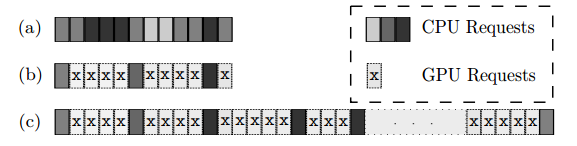
\includegraphics[width = 8 cm]{graphics/no1.png}
	\caption{Limited visibility example due to small buffer size. (a) CPU-only
	case, (b) MC’s visibility when CPU and GPU are combined, (c) Improved
	visibility with a larger request buffer.\cite{SmS}}\label{fig:buff}
\end{figure} 

The increased buffer size does not come without a cost. It increases circuit complexity and results in a significant larger die area. The larger request buffer also leads to higher power consumption and increased costs \cite{SmS} making it an unattractive solution. 

\section{Solutions}
\subsection{Cache line allocation in shared LLC}
The proposed solution is a new cache management policy called HeLM (Heterogeneous LLC Management). It consists on measuring the cache sensitivity of the GPU and CPU, and based on a couple of thresholds decide if GPU access requests to the LLC should be bypassed directly to the main memory or not.
It is based on the fact that GPUs have a much higher TLP than CPUs, and thus are less affected by longer memory access latency. Having a high TLP means that there will most likely be some threads that can be ran while waiting for the memory to respond. If that is the case, bypassing the cache should not affect the IPC count.


To calculate cache sensitivity in the GPUs, set dueling is used. The GPUs TLP is measured as the amount of wavefronts ready to be scheduled. This information is sent along with the LLC access request whenever there is an L1 cache miss. One GPU core is set to do a cache bypass whenever it's TLP is higher than a lowThreshold. Another one is set to do the same but with highThreshold. IPC is measured for both cores and if the difference is higher than pThreshold, the highThreshold is used for the remaining cores.

In the case of the CPUs, the cache misses on the LLC are measured with both lowThreshold and highThreshold bypassing of the GPUs. If the difference in cache misses is higher than mThreshold, the threshold of the GPUs is overridden to be the lowThreshold.

What all this means is that the CPU will be given preference over the GPU in cache allocation. The GPU will be frequently bypassing the LLC cache, specially if its TLP is high. So a penalty in the GPUs IPC is expected. However the CPU IPC is expected to see the most change, since the GPU bypassing of the LLC means the CPU will get more sets for its use.

A comparison to other cache management policies was made with 3 different configurations: 1, 2 and 4 CPU cores, each with 4 GPU cores. A different random benchmark on each CPU core was run, and a random benchmark for all 4 GPUs. For each configuration, the benchmark was changed 100, 40 and 30 times respectively. The reduction of cache misses and speedup was calculated relative to LRU results. Figure~\ref{fig:comp} shows the comparison.

\begin{figure}[H]
	\centering
	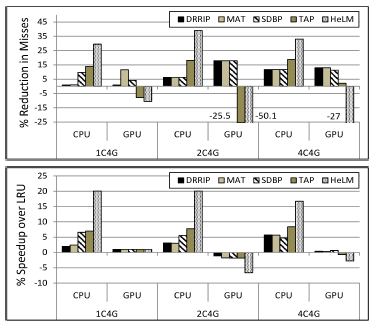
\includegraphics[width = 8 cm]{graphics/LLCresults.png}
	\caption{Percentage reduction in misses and percentage speedup in the CPUs and the GPUs caused by HeLM and other cache management policies in comparison to LRU \cite{LLC}}\label{fig:comp}
\end{figure} 

As can be seen in Figure~\ref{fig:comp} HeLM offer a considerably higher reduction in cache misses and overall speedup for the CPUs. On the GPUs, however, the effect is the opposite, although it is important to notice that a huge increase in misses for the GPU didn't affect so negatively the speedup. To provide a more general overview, the results for CPUs and GPUs were combined into Figure~\ref{fig:comp1}.


\begin{figure}[H]
	\centering
	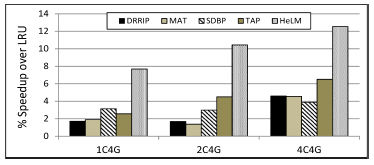
\includegraphics[width = 8 cm]{graphics/LLCresults2.png}
	\caption{Combined percentage speedup of HeLM and other cache management policies in comparison to LRU \cite{LLC}}\label{fig:comp1}
\end{figure} 

Figure~\ref{fig:comp1} shows the overall speedup of HeLM is very noticeable even though it caused a huge amount of misses on the GPU requests. This is because GPU programs are much less sensible to the cache than CPU programs.

\begin{figure}[H]
	\centering
	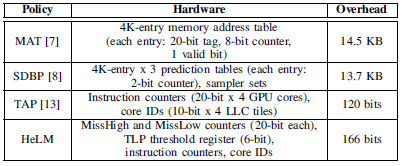
\includegraphics[width = 8 cm]{graphics/LLChardware.png}
	\caption{Hardware overhead of different cache management policies \cite{LLC}}\label{fig:LLChw}
\end{figure}

Finally, a comparison was made on the hardware overhead of HeLM and three other cache management policies. Figure~\ref{fig:LLChw} shows an explanation of the extra hardware needed for each cache policy and a count of the number of flip-flops needed to implement it. As can be seen, the policy with the least overhead is TAP, however it is not a big difference in comparison to HeLM. On the other hand, the speedup achieved by HeLM is considerably higher than TAP.

\subsection{Hybrid-technology memory system}
A proposed solution that addresses the DRAM limitations is a hybrid DRAM/PRAM-based Main Memory. PRAM is a type of non-volatile RAM which stores information as phase-state in a cell. The PRAM’s main advantages over DRAM  are the better-scaling projections and the low idle-power consumption. However, because of the low writing endurance and high-latency for writes, the technology is not a valid replacement for DRAM, being best suited to complement it in the critical points (storage and power consumption).

Combining the benefits of the two technologies, the authors proposed two types of the hybrid system that can hide their weak points. 
\begin{figure}
	\centering
	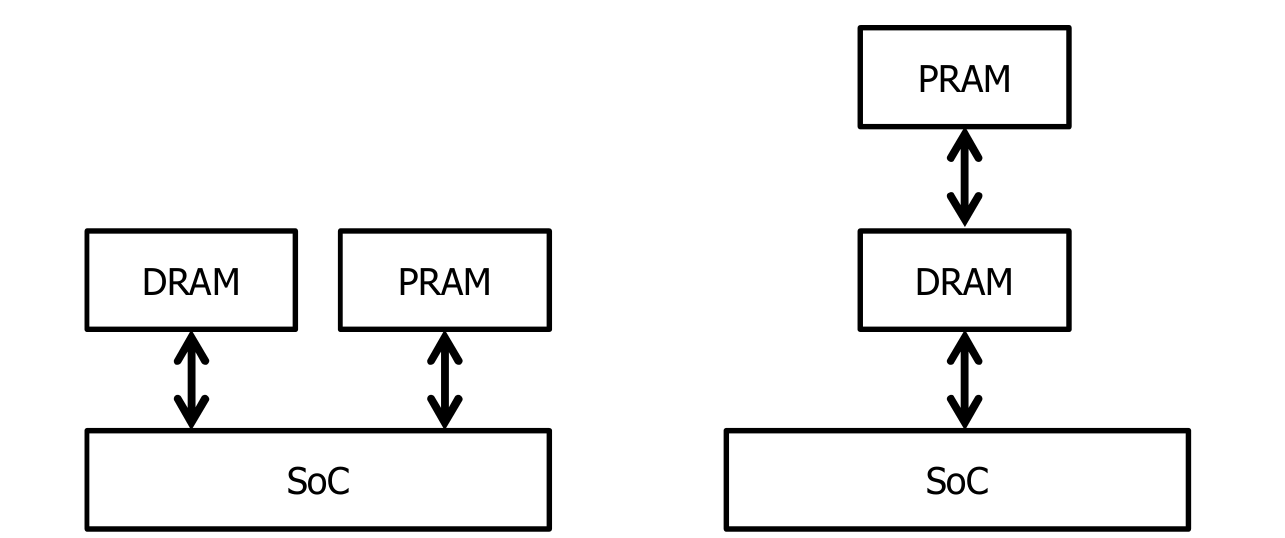
\includegraphics[width = 8 cm]{graphics/structure-hybrid.png}
	\caption{(a) Flat structure (b) Hierarchical structure}\label{fig:buff}
\end{figure} 
First variant is a hierarchical-topology organization, where the DRAM plays the role of a Last-Level Cache and the PRAM is the main memory. However, when regarding the CPU’s needs, a LLC miss would involve a very high latency for fetching the needed data from the main memory. In the projected case, 40 us for retrieving unused data from the PRAM transforms into 40.000 cycles for a 1 GHz CPU, an overhead too big for any out-of-order execution mechanism, assuring a deep stall on every processing unit, thus considerably reducing the IPC count.

The second approach is a flat organization of the two technologies, with the DRAM mainly serving the CPU purposes, and the PRAM meant for the GPU side. This kind of implementation has several advantages over the hierarchical:
\begin{itemize}
\item{It eliminates the issue of very high miss penalty on the LLC (DRAM for that proposal).}
\item{It separates the memory-buses, avoiding possible GPU-CPU conflicts in critical points, such as the synchronization of complex CPU applications with memory-hungry GPU activity.}
\end{itemize}
\begin{figure}[H]
	\centering
	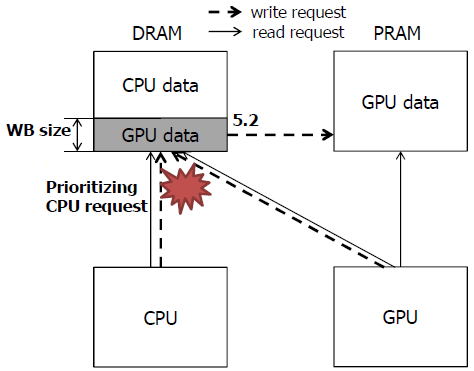
\includegraphics[width = 8 cm]{graphics/StructureWithBuffer.PNG}
	\caption{Overall view of the proposed hybrid structure with hot-write DRAM buffer}\label{fig:buff}
\end{figure} 
However, having the GPU working only with the PRAM memory can result in missing deadlines (because of the high write-latency), when write-intensive applications are under execution. Therefore, a dynamic hot-write buffer has been created in the DRAM memory to handle successive write requests to GPU main memory. Furthermore, the hot-write buffer removes the issue of cell wear by reducing the number of writes to a single bit (also by implementing the differential writing mechanism), thus expanding the PRAM's lifetime and reliability.

\subsection{Staged memory scheduling}
The proposed solution is a new memory controller (MC), Staged Memory Scheduling (SMS),  that is a simpler implementation in hardware and provides performance and fairness improvements over the application-aware MC.  It is split into three stages, the batch formation, batch scheduler and a DRAM command scheduler.

\begin{figure}[H]
	\centering
	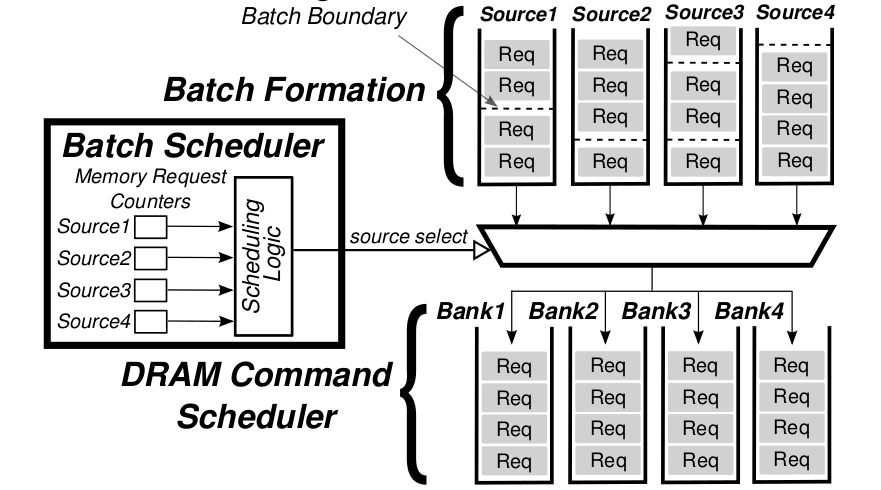
\includegraphics[width = 8 cm]{graphics/SmS.png}
	\caption{organization of the SMS \cite{SmS}}
\end{figure}

The batch formation is focused on row-buffer locality.  It groups together requests from applications that want to access the same row in the main memory. The second stage , the batch scheduler, schedules batches from different applications and the third stage, the DRAM Command Scheduler schedules requests while satisfying all DRAM constrains \cite{SmS}

Stage 1: Is built from simple FIFO structures that have one structure per sources.  One source is a single CPU-core or the GPU.  One batch is one or more memory requests from the same source that request access to the same DRAM row.  A batch is only ready when a request to a new DRAM row comes in, it is full or when the oldest request in the batch has exceeded a predefined age threshold.  A batch that is considered ready moves to stage 2 the Batch scheduler.

Stage 2:  The Batch Scheduler operates in two states, the pick  and the  drain.  In the pick state in picks a batch from stage 1 and than enters drain state where it feeds the FIFO batch to DRAM Command Scheduler one request per clock cycle until the whole batch is gone.  The picking is done in one of two fashions.  It picks the batch using either round-robin policy or shortest job first (SJF).   SJF tends to favor latency-sensitive applications that tend to have fewer total requests and thus favoring the CPU over the GPU.  On the other hand the round-robin simply picks the next ready batch in a round-robin manner and thus servicing high memory-intensive applications and favoring the GPU over the CPU.  The batch scheduler uses SJF with a probability of $p$ and round-robin  $ 1 - p $ which will be explained better later.

Stage 3: DRAM Command Scheduler (DCS) consists of few FIFO queues or one per DRAM bank.  Since the row-buffer locality from stage 1 has been preserved the only job of the DCS is to issue low-level DRAM commands and ensuring DRAM protocol compliance. 

Some batches bypass stage 1 and 2 and go directly to the DCS. Latency-sensitive requests of applications with low memory-intensity and all requests wen the system is lightly loaded, that is when total number of in-flight requests over all sources in the DCS are fewer the 16.\\

The probability parameter $p$:  As stated above the probability of SJF used is $p$ and that of round-robin policy $1-p$.  Therefor the value of $p$ determines  which gets higher priority, the CPU or the
GPU.  That is when $p$ is high the SJF policy is performed more frequently then round-robin and therefore favoring less memory-intensive applications of the CPU over the GPU.  And on the other hand when p is low request batches are scheduled more often in round-robin fashion favoring memory-intensive applications of the GPU over the CPU.  As different systems have different performance needs it is proposed to have $p$ a dynamic parameter that can be tuned to the needs of different systems.\\

\textbf{Hardware Implementation}
Batch Formation:  The hardware implementation for stage can be of a fairly simple nature as it only needs one comparator per source.  A new request has only to be checked if it can fit in the existing batch or not.  That is if the incoming request row index is the same as the last request that entered the batch.  The hardware overhead can be seen in Table \ref{tab:SmS1}

\begin{table}[H]
  \centering
  \resizebox{14.3 cm}{!}{\begin{minipage}{\textwidth}
	\begin{tabular}{| l | l |}
		\hline
		Storgae & Size \\ \hline
		CPU FIFO queues 			& $N_{core} × Queue\_Size_{core} = 160 entries$ 					\\\hline
		GPU FIFO queues 			& $N_{GPU} × Queue\_Size_{GPU} = 20 entries$ 						\\\hline
		MPKC counters   			& $N_{core} × log_2 MPKC_{max} = 160 bits$							\\\hline
		Last request’s row index	& $(N_{core} + N_{GPU} ) × log_2\_ Row\_ Index\_ Size = 204 bits$ 	\\\hline
	\end{tabular}
	
  \end{minipage} }
  \caption{Storage Overhead of Stage 1: Batch formation stage \cite{SmS}}\label{tab:SmS1}
\end{table}

Batch Scheduler:  The batch scheduler does not need to be very complex as it only schedules FIFOS that are as many as there are sources or cores.  When SJF is applied a tree of MIN operators can be build from the out standing batches.  As the batches are not many the tree will not get very large. The hardware overhead can be seen in Table \ref{tab:SmS2}

\begin{table}[H]
  \centering
  \resizebox{15.5 cm}{!}{\begin{minipage}{\textwidth}
	\begin{tabular}{| l | l |}
		\hline
		Storgae & Size \\ \hline
		CPU memory request counters 			& $N_{core} × log_2 Count_{max\_CPU} = 80 bits$ 					\\\hline
		GPU memory request counter 			& $N_{GPU} × log_2 Count_{max\_GPU} = 10 bits$ 						\\\hline	
	\end{tabular}
  \end{minipage} }
  \caption{Storage Overhead of Stage 2: Batch Schedule \cite{SmS}}\label{tab:SmS2}
\end{table}

DRAM Command Scheduler:   Compared to the monolithic scheduler the DRAM command scheduler is on completely different scale.  It consist of per-bank FIFOs, eight per rank for DDR3, and only needs to look at the head of one. The hardware overhead can be seen in Table \ref{tab:SmS3}

\begin{table}[H]
  \centering
  \resizebox{17 cm}{!}{\begin{minipage}{\textwidth}
	\begin{tabular}{| l | l |}
		\hline
		Storgae & Size \\ \hline
		Per-Bank FIFO queues			& $N_{banks} × Queue\_Size_{bank} = 120 entries$ 					\\\hline
	\end{tabular}
  \end{minipage} }
  \caption{Storage Overhead of Stage 3: DRAM Command Scheduler \cite{SmS}}\label{tab:SmS3}
\end{table}
The hardware required for the SMS is summarized in Table~\ref{fig:SMSTable}

\section{Comparisons}
\subsection{Hybrid memory system}
Regarding the baseline in \cite{PRAM}, although the improvements in energy consumption and memory size constraints do matter, a PRAM-only main memory system shows significant slowdowns for a regular SoC. The performance overhead is in average about 40 \% making it not suitable for deployment in current computer architecture designs. 

For tackling the big overhead issue, the hybrid system has been proposed. 

The PRAM/DRAM main memory system significantly improves performance for the GPU, with small overhead on the CPU side. As presented in the experiments, the improvement over an uniform PRAM main memory is in average 24, using the DL+CM memory management for the hot-write buffer. However, the reduction in CPU IPC can go up to 33 \% \cite{PRAM}for the SL+CM and 23.6 \% with the DL+CM, taking in account a 8K entries (64B per entry) buffer. 

Regarding the energy consumption constraints, the proposed solution show savings ranging from 12 to 50 \% in comparison with the DRAM-only main memory baseline system\cite{PDRAM}.
\section{Perspectives}
Write here perspectives (maybe of our own ideas). 

\section{Conclusion}
Drop the memory. It's slow anyway

% use section* for acknowledgement
\ifCLASSOPTIONcompsoc

% Can use something like this to put references on a page
% by themselves when using endfloat and the captionsoff option.
\ifCLASSOPTIONcaptionsoff
  \newpage
\fi

\bibliographystyle{IEEEtran}

\bibliography{ref}

\newpage

% that's all folks
\end{document}
